\item[]\textbf{Questão 10}

\hspace{1cm}O principal ensaio realizado é o de Proctor. Por meio do traçado da ``curva de compactação'' é possível estabelecer a umidade que fornece melhor qualidade mecânica ao solo e, dessa forma, sob mesma energia de compactação determinar a resistência da amostra. 

Os parâmetros essenciais que devem ser fornecidos no laboratório são:

\begin{enumerate}
	\item[1.] Peso aparente seco
	\item[2.] Umidade da amostra
\end{enumerate}

Com base nesses dados é traçada 

\begin{figure}[h!]
	\centering
	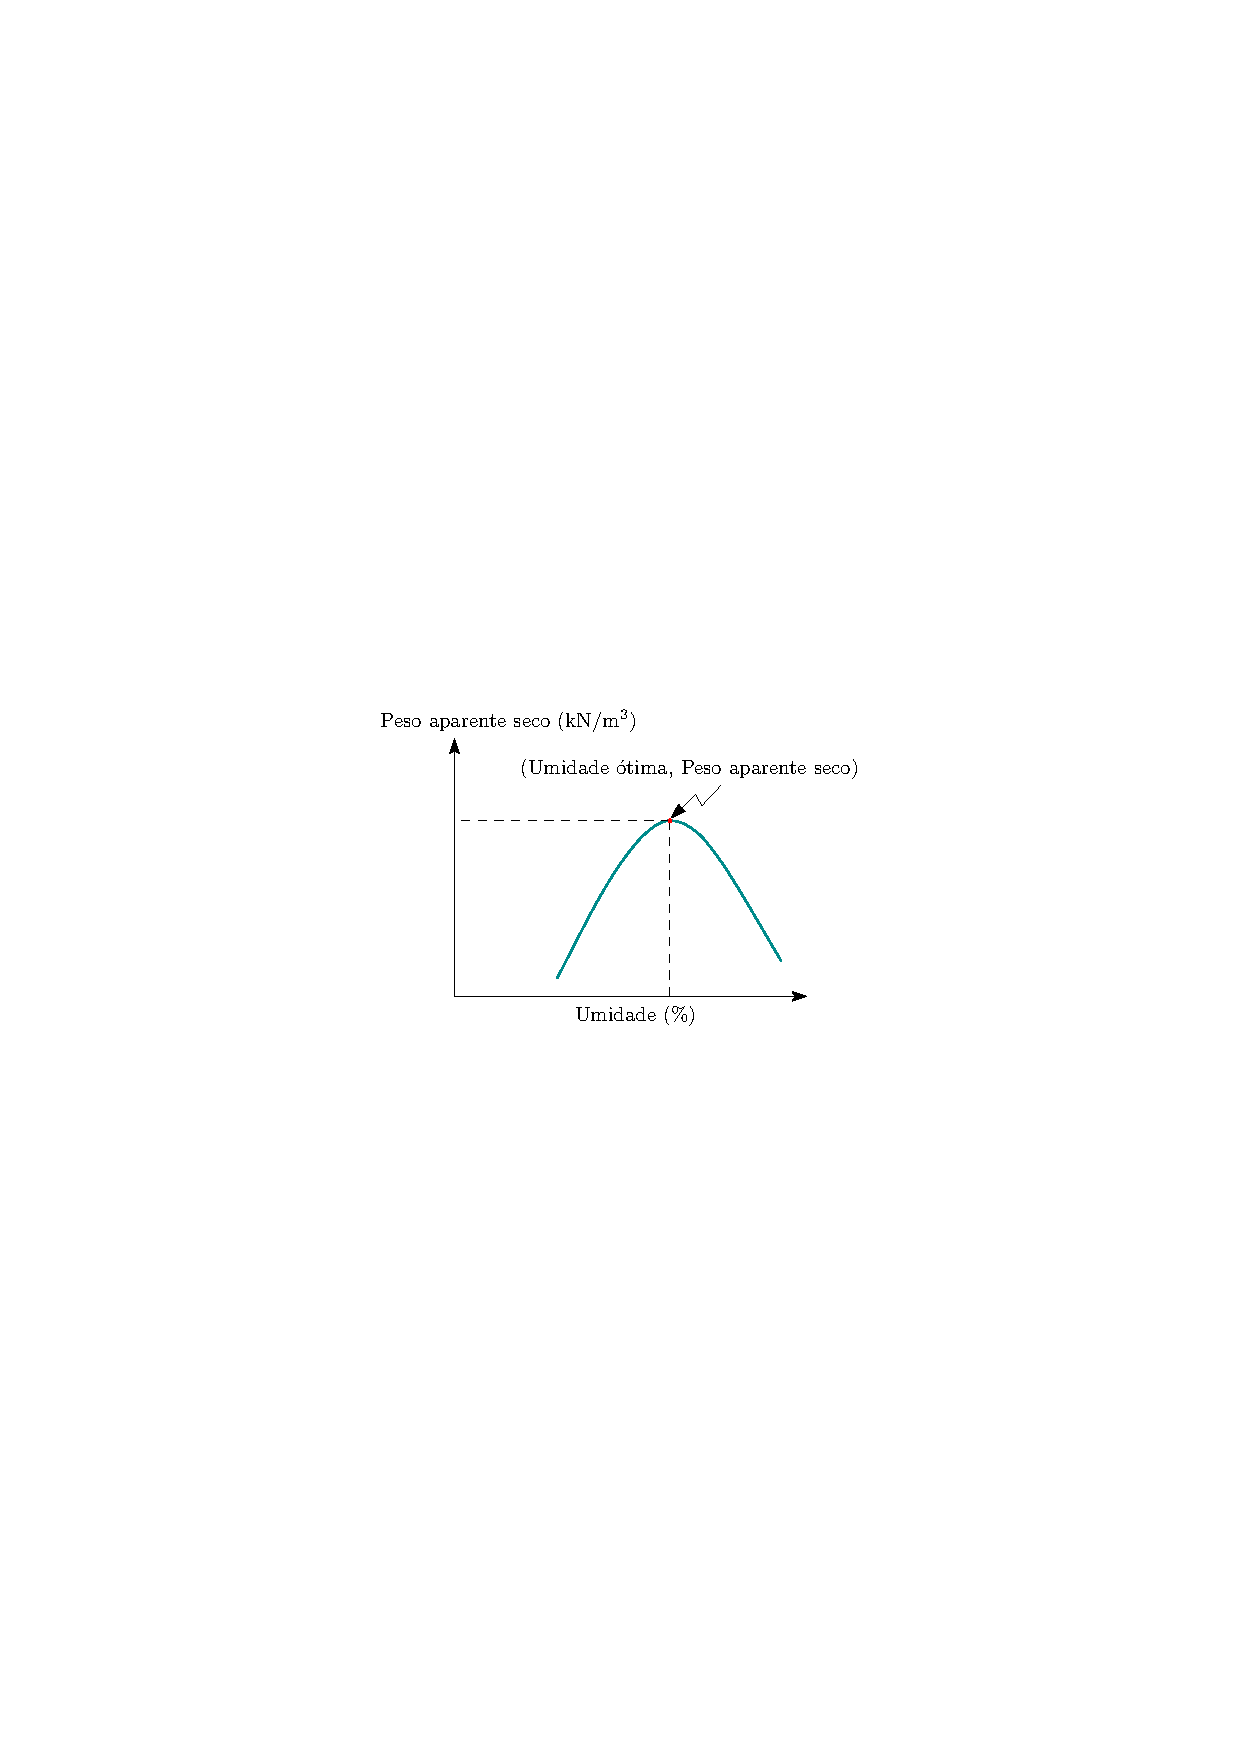
\includegraphics[scale=1.2]{images/proctor}
\end{figure}